\subsection{Correctness at moderate size}\label{subsec:correct}
Table~\ref{tab:e1} runs every family at a size where the dense reference is affordable. In all
cases the residual is at the level of rounding, the solver error is a small multiple of
$\kappa(H)\,u$, and the null-space fraction (the part of $x$ that a minimum-norm solution must not
have) is of the same order as the solver error. That last point matters: an algorithm that solved
$Hx=b$ but drifted from the minimum-norm solution would show a null-space fraction far above the
residual. The ``vs.\ $A$'' column adds the compression error and tracks the ID tolerance
($10^{-10}$--$10^{-12}$), consistent with the $\approx2\kappa\varepsilon$ bound. For F6 the end-to-end
error in the \emph{Toeplitz} variables is $1.6\times10^{-12}$, after mapping back with $x=D^*F_n^*y$.
The HSS rank of the random Toeplitz matrix itself is 512 (incompressible), against 62 for its
Cauchy-like transform.

\begin{table}[!htb]
\centering\scriptsize
\setlength{\tabcolsep}{3pt}
\begin{tabular}{@{}lrrrrrcccccc@{}}
\toprule
case & $m$ & $n$ & $L$ & rank & $\kappa(H)$ & As.~\ref{as:slack} & residual & solver error & null frac. & vs.\ $A$\\
\midrule
F1 & 320 & 480 & 4 & 3 & $1.3{\times}10^{3}$ & yes & $5.9{\times}10^{-15}$ & $2.3{\times}10^{-14}$ & $1.6{\times}10^{-14}$ & $2.3{\times}10^{-14}$\\
F1 & 2048 & 4096 & 7 & 3 & $7.4{\times}10^{3}$ & yes & $2.8{\times}10^{-14}$ & $1.9{\times}10^{-13}$ & $1.7{\times}10^{-13}$ & $1.9{\times}10^{-13}$\\
F2 & 1024 & 2048 & 5 & 10 & 14 & yes & $1.4{\times}10^{-15}$ & $3.6{\times}10^{-15}$ & $3.2{\times}10^{-15}$ & $3.6{\times}10^{-15}$\\
F2 complex & 1024 & 2048 & 5 & 10 & 13 & yes & $1.5{\times}10^{-15}$ & $5.2{\times}10^{-15}$ & $4.6{\times}10^{-15}$ & $5.2{\times}10^{-15}$\\
F2 $m/n=0.9$ & 1800 & 2000 & 5 & 8 & 79 & no & $2.5{\times}10^{-15}$ & $1.4{\times}10^{-14}$ & $1.2{\times}10^{-14}$ & $1.4{\times}10^{-14}$\\
F3 & 1024 & 3069 & 5 & 32 & 1.9 & yes & $1.1{\times}10^{-15}$ & $2.2{\times}10^{-15}$ & $2.2{\times}10^{-15}$ & $6.7{\times}10^{-11}$\\
F4 Gaussian, $\sigma=2$, $s=2$ & 2040 & 4096 & 5 & 10 & 98 & yes & $6.6{\times}10^{-15}$ & $1.0{\times}10^{-14}$ & $8.7{\times}10^{-15}$ & $1.0{\times}10^{-14}$\\
F4 Ricker, $\sigma=3$, $s=2$ & 2036 & 4096 & 5 & 15 & $2.2{\times}10^{3}$ & yes & $7.7{\times}10^{-14}$ & $1.9{\times}10^{-13}$ & $1.9{\times}10^{-13}$ & $2.0{\times}10^{-13}$\\
F4 Gaussian, $\sigma=3$, $s=3$ & 1358 & 4096 & 5 & 10 & 98 & yes & $5.1{\times}10^{-15}$ & $1.0{\times}10^{-14}$ & $9.3{\times}10^{-15}$ & $1.0{\times}10^{-14}$\\
F5 & 1536 & 2048 & 5 & 36 & 2.0 & no & $1.2{\times}10^{-15}$ & $3.1{\times}10^{-15}$ & $3.1{\times}10^{-15}$ & $1.0{\times}10^{-12}$\\
F6 & 1024 & 2048 & 5 & 62 & 7.4 & no & $2.1{\times}10^{-15}$ & $4.2{\times}10^{-15}$ & $3.7{\times}10^{-15}$ & $1.4{\times}10^{-12}$\\
\bottomrule
\end{tabular}

\caption{E1, solver error against the dense minimum-norm solution of the same HSS matrix
(relaxed rule, as in the current solver; the legacy rule, \texttt{slack='collapse'}, which merges a level in the
F2 $m/n=0.9$, F5 and F6 cases, gives errors of the same size). ``rank'' is the largest
generator rank, $L$ the depth.}
\label{tab:e1}
\end{table}

\subsection{Stability against conditioning}\label{subsec:stab}
Figure~\ref{fig:stab} sweeps $\kappa(H)$ in two exact-HSS families: F2 with random column grading,
up to $\kappa\approx7\times10^{12}$ (depth 3), and the ``valid'' Gaussian blur, up to $\kappa\approx10^8$
(depth 4). The reference is computed with 60 digits, and all solvers see the same matrix. The ULV
solve with a factored root solve (blue; the current solver) tracks the backward-stable dense QR solve over the whole
range: forward error $\approx\kappa u$ and backward error $\approx u$. It is even slightly more accurate than
dense QR at the largest $\kappa$. The normal equations follow $\kappa^2u$ and have lost all accuracy by
$\kappa\approx10^8$ (beyond it Cholesky fails). CG on $HH^*$ (CGNE) does not converge within 2000
iterations once $\kappa\gtrsim6\times10^2$ (blur) to $9\times10^3$ (graded). This is the practical case for a
direct ULV solver over the normal-equation approaches the repo tried before (\texttt{hss\_udsolve},
\texttt{ud\_normeqs\_pcg}). Column grading is used because it keeps the matrix \emph{exactly} HSS at
every $\kappa$; replacing the singular values of an SVD, as the earlier \texttt{june2026} sweep does,
changes the off-diagonal ranks. Panel (c) repeats the graded test on a $2048\times4096$ matrix with a
depth-6 tree, against dense QR (a 60-digit reference is out of reach at that size). The ULV backward error
stays at or below $1.9\times10^{-16}$ up to $\kappa\approx10^{14}$, and the difference from QR stays below $\kappa u$.

\paragraph{The root solve.} The red curves use the legacy root solve, \texttt{pinv(D)*b}, which forms the
pseudo-inverse explicitly (reproduced in the port with \texttt{root='pinv'}). For the blur family its
backward error grows with $\kappa$, to $10^{-12}$--$3\times10^{-12}$ for $\kappa\ge6\times10^7$, while the forward
error is unchanged. The cause is classical~\cite{higham}: the computed $X=D^++E$ has
$\|E\|=O(u\|D^+\|)$, so the residual $DEb$ can be as large as $u\,\kappa(D)\|b\|$. A backward-stable solve
leaves a residual $O(u(\|D\|\|x\|+\|b\|))$, which is smaller by up to $\kappa(D)$ when $b$ lies mostly
along the large singular directions. In the blur family the root block carries most of $\kappa(H)$
($\operatorname{cond}(D)=10^5$ at $\kappa=1.5\times10^5$, $4\times10^7$ at $\kappa=10^8$). In the graded family the
grading is absorbed by the leaf-level triangular solves and the root stays well conditioned
($\operatorname{cond}(D)\le4$ in panel c), so the two root solves agree there. The MATLAB files
behave the same way. Under Octave, on four blur matrices with $\kappa=1.5\times10^5$--$1.1\times10^8$, the
legacy \texttt{H\textbackslash b} has backward errors of $1.5\times10^{-14}$--$2.5\times10^{-12}$. The current
\texttt{H\textbackslash b}, which applies the SVD factors to $b$, gives $1.6$--$2.4\times10^{-16}$ on the same
matrices. In the MATLAB suite, \texttt{mp\_exp\_conditioning} reports the current solver's backward error and
\texttt{mp\_test\_solver} checks it on two of these matrices. The fix costs nothing (Section~\ref{sec:open}).
\emph{Scope:} these are empirical statements for trees of depth 3--6 and $\kappa$ up to $10^{14}$; no
backward-error bound is proved.

\begin{figure}[!htb]
\centering
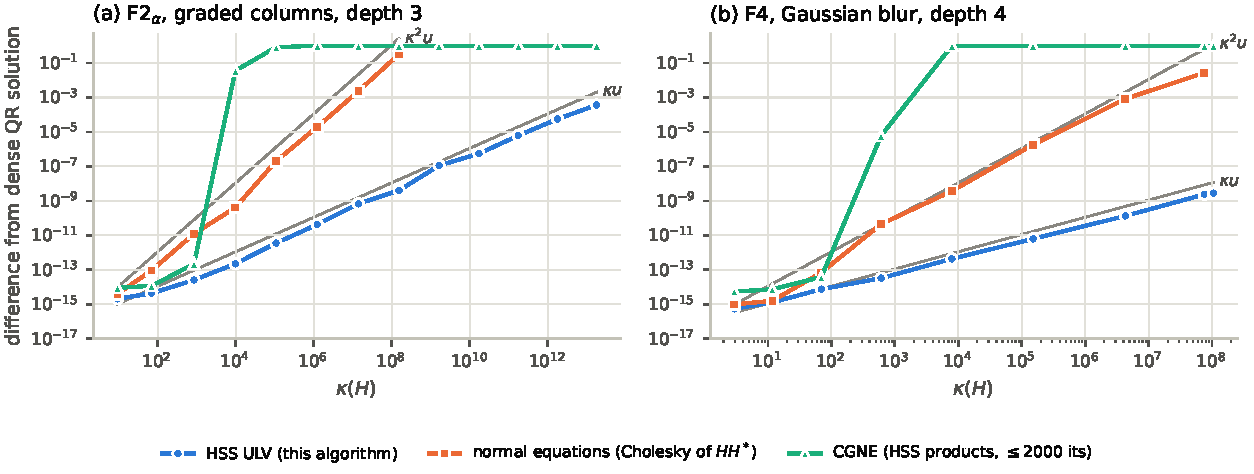
\includegraphics[width=\textwidth]{figures/m1_stability.pdf}
\caption{E2, stability. Top: forward error against a 60-digit reference ((c): difference from dense
QR). Bottom: normwise backward error. Grey lines: $\kappa u$, $\kappa^2u$, $u$. $128\times256$ (a),
$\approx290\times300$ (b) and $2048\times4096$ (c), all exactly HSS. Blue: factored root solve (current solver). Red:
explicit \texttt{pinv} at the root (legacy file); in (a) and (c) it coincides with blue.}
\label{fig:stab}
\end{figure}

\subsection{Large-scale accuracy}\label{subsec:large}
With manufactured solutions the solver can be checked at sizes where no dense matrix fits
(Figure~\ref{fig:largescale}). For F2--F5 the error stays flat at $1$--$4\times10^{-15}$ from $n=2^{10}$
to the largest size: $2^{20}$ for F2, $\approx5\times10^5$ for F3 and F4, $2.6\times10^5$ for F5. For F1
it grows from $10^{-13}$ to $10^{-10}$, in step with $\kappa(\text{F1})\propto n$; that is the
conditioning of the test matrix, not error growth in the solver. Residuals are
$\lesssim10^{-15}$ throughout (largest $1.2\times10^{-15}$).

\begin{figure}[!htb]
\centering
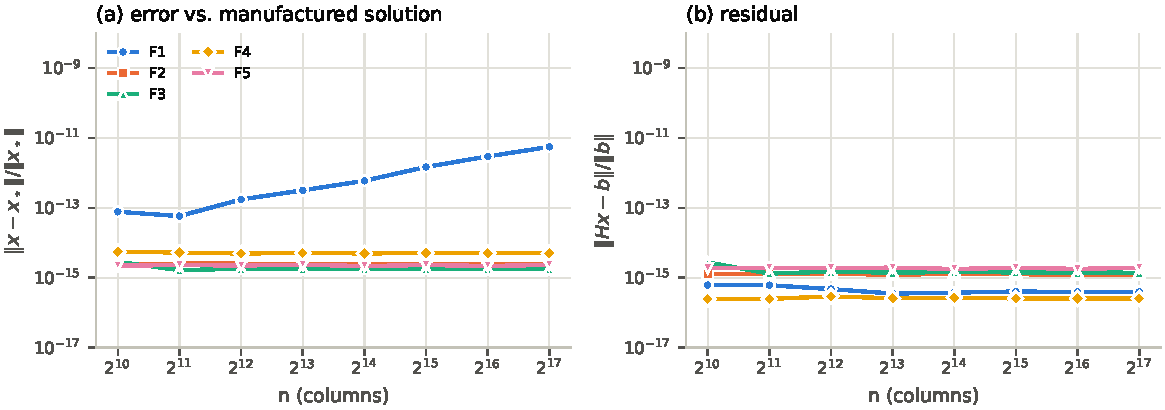
\includegraphics[width=0.78\textwidth]{figures/m1_largescale_accuracy.pdf}
\caption{E3, error against the manufactured minimum-norm solution and residual, up to
$n=2^{20}$. No dense matrix is formed.}
\label{fig:largescale}
\end{figure}

\subsection{Timing and scaling}\label{subsec:timing}
Figure~\ref{fig:timing} and Table~\ref{tab:scaling} show factorization and solve times. The fitted
slopes over the last four sizes are $0.96$--$1.17$, so the cost is linear in $n$ as
Section~\ref{sec:complexity} predicts. A million columns factor in about 10\,s single-threaded
(F1, F2). A solve that reuses the factors is $4$--$16\times$ cheaper than a factorization at the
largest sizes ($3$--$23\times$ over all sizes; the ratio grows with the rank). The dense QR min-norm
solve scales like $n^{3.06}$. The HSS solve is already faster at $n=512$ and is $177\times$ faster at
$n=8192$. CGNE needs 90--182 iterations even at $\kappa\approx10$ and is 3--8$\times$ slower than the
direct solve there; it fails outright for ill-conditioned problems (Section~\ref{subsec:stab}).

\begin{figure}[!htb]
\centering
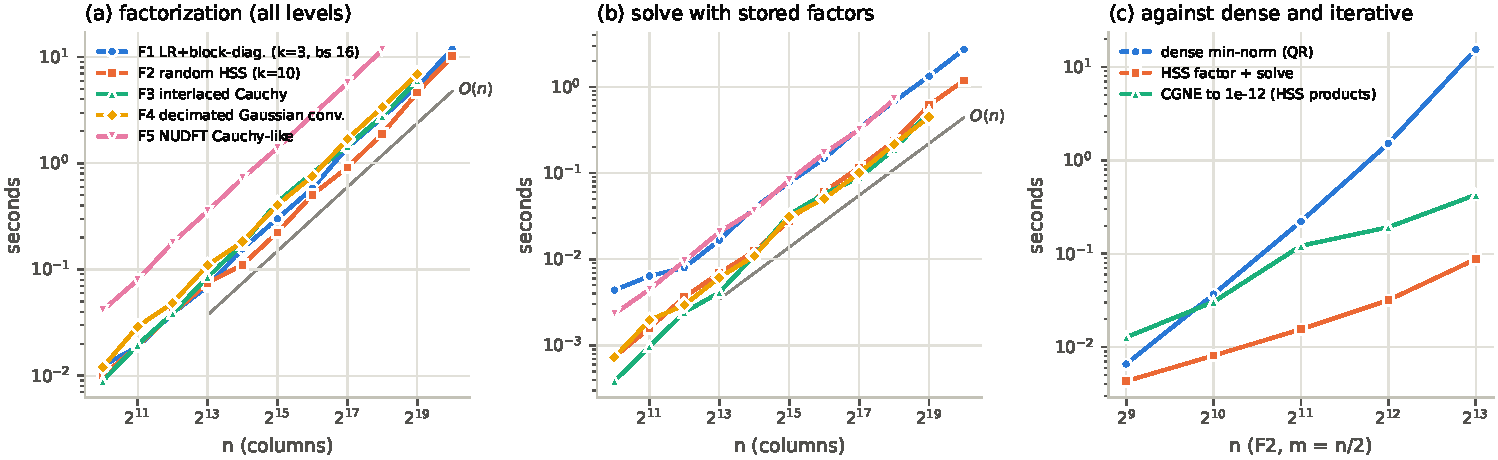
\includegraphics[width=\textwidth]{figures/m1_timing.pdf}
\caption{E4, single-threaded time (median of 5, or of 3 for $n\ge2^{17}$). (a) Full factorization;
(b) solve with stored factors; (c) against dense QR and CGNE (F2, $m=n/2$). Grey: $O(n)$.}
\label{fig:timing}
\end{figure}

\begin{table}[!htb]
\centering\small
\begin{tabular}{@{}lrrrrrrr@{}}
\toprule
family & largest $n$ & rank & build (s) & factor (s) & solve (s) & slope & max error\\
\midrule
F1 LR+block-diag. & 1048576 & 3 & -- & 11.83 & 2.72 & 1.02 & $1.3{\times}10^{-10}$\\
F2 random HSS & 1048576 & 10 & -- & 10.21 & 1.19 & 1.17 & $1.5{\times}10^{-15}$\\
F3 Cauchy (proxy) & 524286 & 42 & 26.0 & 6.01 & 0.51 & 0.96 & $1.2{\times}10^{-15}$\\
F4 conv. (proxy) & 524288 & 10 & 10.3 & 6.91 & 0.45 & 1.06 & $4.1{\times}10^{-15}$\\
F5 NUDFT (proxy) & 262144 & 50 & 27.9 & 11.69 & 0.72 & 1.02 & $1.5{\times}10^{-15}$\\
\bottomrule
\end{tabular}

\caption{Largest sizes reached. ``build'' is the $O(n)$ proxy construction. ``slope'' is the
least-squares exponent of factor time over the last four sizes.}
\label{tab:scaling}
\end{table}

\subsection{Rank, blocksize, aspect ratio, and the slack assumption}\label{subsec:sweeps}
Figure~\ref{fig:sweeps}. (a) Rank, F2, $n=2^{16}$, $m=n/2$, at two fixed leaf sizes ($64\times128$ and
$128\times256$). The flop count of Section~\ref{sec:complexity} (\texttt{hssmn.cost}: the dense kernels of
every node at every level), scaled once per leaf size, matches the measured times to within 21\%
($n_0=64$) and 13\% ($n_0=128$). The cost is nearly flat while $k\ll n_0$ and rises once
$k\gtrsim n_0/2$, where the reduced levels ($2k\times4k$ nodes) become as large as the leaves. One scale
per leaf size is needed because the larger blocks run at a higher flop rate (10 against
6\,GFlop/s). (b) The best blocksize is 32--64 for $k=10$. Smaller leaves pay
per-node overhead, larger leaves pay $p_0n_0^2$. (c) Aspect ratio, $k=16$, blocksize 64.
Assumption~\ref{as:slack} fails at $m/n\ge0.9$ (leaf slack $p_\tau-n_\tau<\ell_\tau$). The legacy rule,
simulated in the Python port (\texttt{slack='collapse'}), then merges one level (at 0.9) or two (at
0.95), always before the first level is processed (Section~\ref{subsec:merge}). That costs
$1.7\times$ and $4.2\times$ the relaxed rule, with the same accuracy: each merge doubles the leaf size,
and the leaf work grows $\approx4\times$ per merge. With higher ranks or smaller blocksizes the collapse
cascades further. For a square matrix ($m/n=1$) the legacy rule would merge every level and end in a dense
$16384\times16384$ \texttt{pinv}; the legacy \texttt{H\textbackslash b} avoided this only because it sent square
systems to a separate square solver. The current \texttt{H\textbackslash b} uses the relaxed rule for square $H$
too; with it the Python port solves the square system in 0.19\,s with error $5\times10^{-13}$.

\begin{figure}[!htb]
\centering
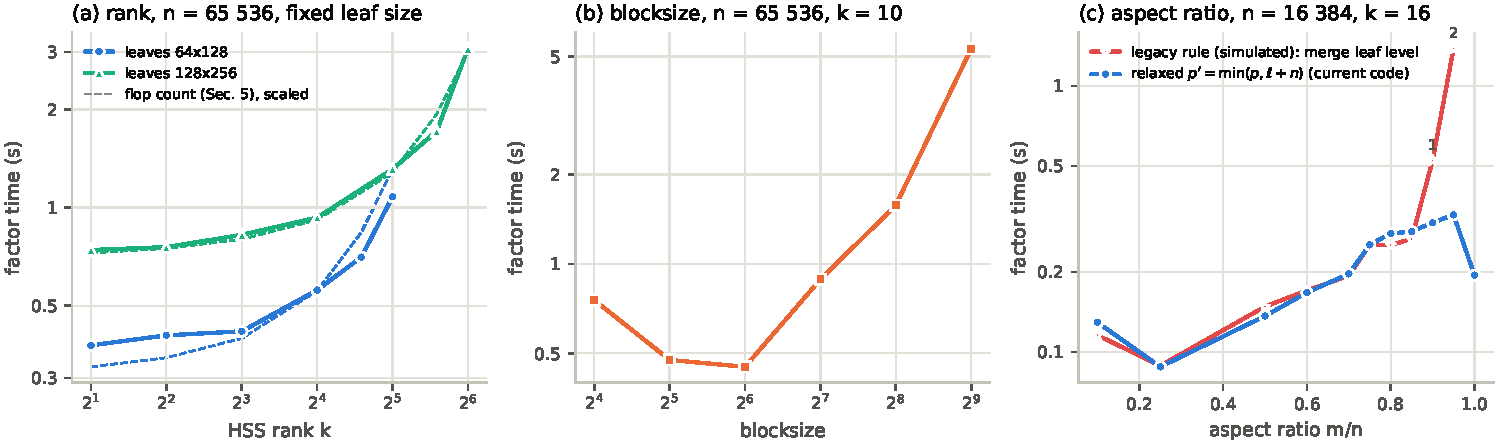
\includegraphics[width=\textwidth]{figures/m1_sweeps.pdf}
\caption{E5/E6, sweeps. (a) Dashed: flop count of Section~\ref{sec:complexity}, scaled once per leaf size. Numbers in (c) are the levels merged by the legacy slack rule (simulated in Python).}
\label{fig:sweeps}
\end{figure}
